\documentclass[a4paper, 11pt]{scrartcl}

%% Language and font encodings
\usepackage[english]{babel}
\usepackage[utf8x]{inputenc}


%% Sets page size and margins
\usepackage[a4paper,top=3cm,bottom=2cm,left=3cm,right=3cm,marginparwidth=1.75cm]{geometry}

%% Useful packages
\usepackage{amsmath}
\usepackage{graphicx}
\usepackage{float}
\usepackage{url}
\usepackage{listings}
\usepackage[colorinlistoftodos]{todonotes}
\usepackage[colorlinks=true, allcolors=blue]{hyperref}

\usepackage{authblk}

\lstdefinelanguage{F}{%
	language     = C,
	morekeywords = {fract},
	basicstyle=\ttfamily,
	keywordstyle=\color{blue}\ttfamily,
	stringstyle=\color{red}\ttfamily,
	commentstyle=\color{gray}\ttfamily,
	morecomment=[l][\color{magenta}]{\#}
}

\title{FAC - F Accademic Compiler}
\author[1]{Mirko Bez}
\author[2]{Stefano Munari}
\affil[1]{\href{mailto:mirko.bez@studenti.unipd.it}{mirko.bez@studenti.unipd.it}}
\affil[2]{\href{mailto:stefano.munari.1@studenti.unipd.it}{stefano.munari.1@studenti.unipd.it}}

% Image directory
\graphicspath{{res/img/}}
% Set path for the sections
\makeatletter
\providecommand*{\input@path}{}
\g@addto@macro\input@path{{section/}}% append
\makeatother


\begin{document}
\maketitle
\tableofcontents
\listoffigures
\lstlistoflistings
\newpage
\section*{Introduction}

FAC is the front end part of a compiler which translates programs written in the
F language into a target representation. FAC is written in C using
flex \cite{flex-online} and bison \cite{bison-online}.
It is interesting to note that FAC can potentially support many target
representations.

\subsection*{Architecture}
Fig. \ref{fig:arch-ovw} describes the architecture of FAC.
Its high-level structure is formed by two macro components:
\begin{itemize}
\item Lexer - the lexical analyzer;
\item Parser - which is divided into three parts:
\begin{itemize}
	\item Syntax analysis;
	\item Static semantic analysis;
	\item Target code generation.
\end{itemize}
\end{itemize}

FAC has been written to be modular. Indeed, it is possible to translate any F
program into other representations simply by writing a new printer implementation.
\\
In FAC a printer is a component which takes the three address code (3AC) of an F
program given as input and generates a version of that code translated into a targeted
representation.
\\
Currently, FAC supports three printers:
\begin{itemize}
\item IR (Internal Representation) - useful for educational purposes or to quickly debug the 3AC;
\item C - prints a C program;
\item Java\footnote{For time reasons only the skeleton has been implemented.} - prints a Java program.
\end{itemize}

We chose to use two different intermediate representations:
\begin{itemize}
\item Abstract Syntax Three (AST) - because it is easy to perform semantic analysis on this structure;
\item Three Address Code (3AC) - because it is easy to perform code generation by parsing this structure.
\end{itemize}

\begin{figure}[H]
  \centering
  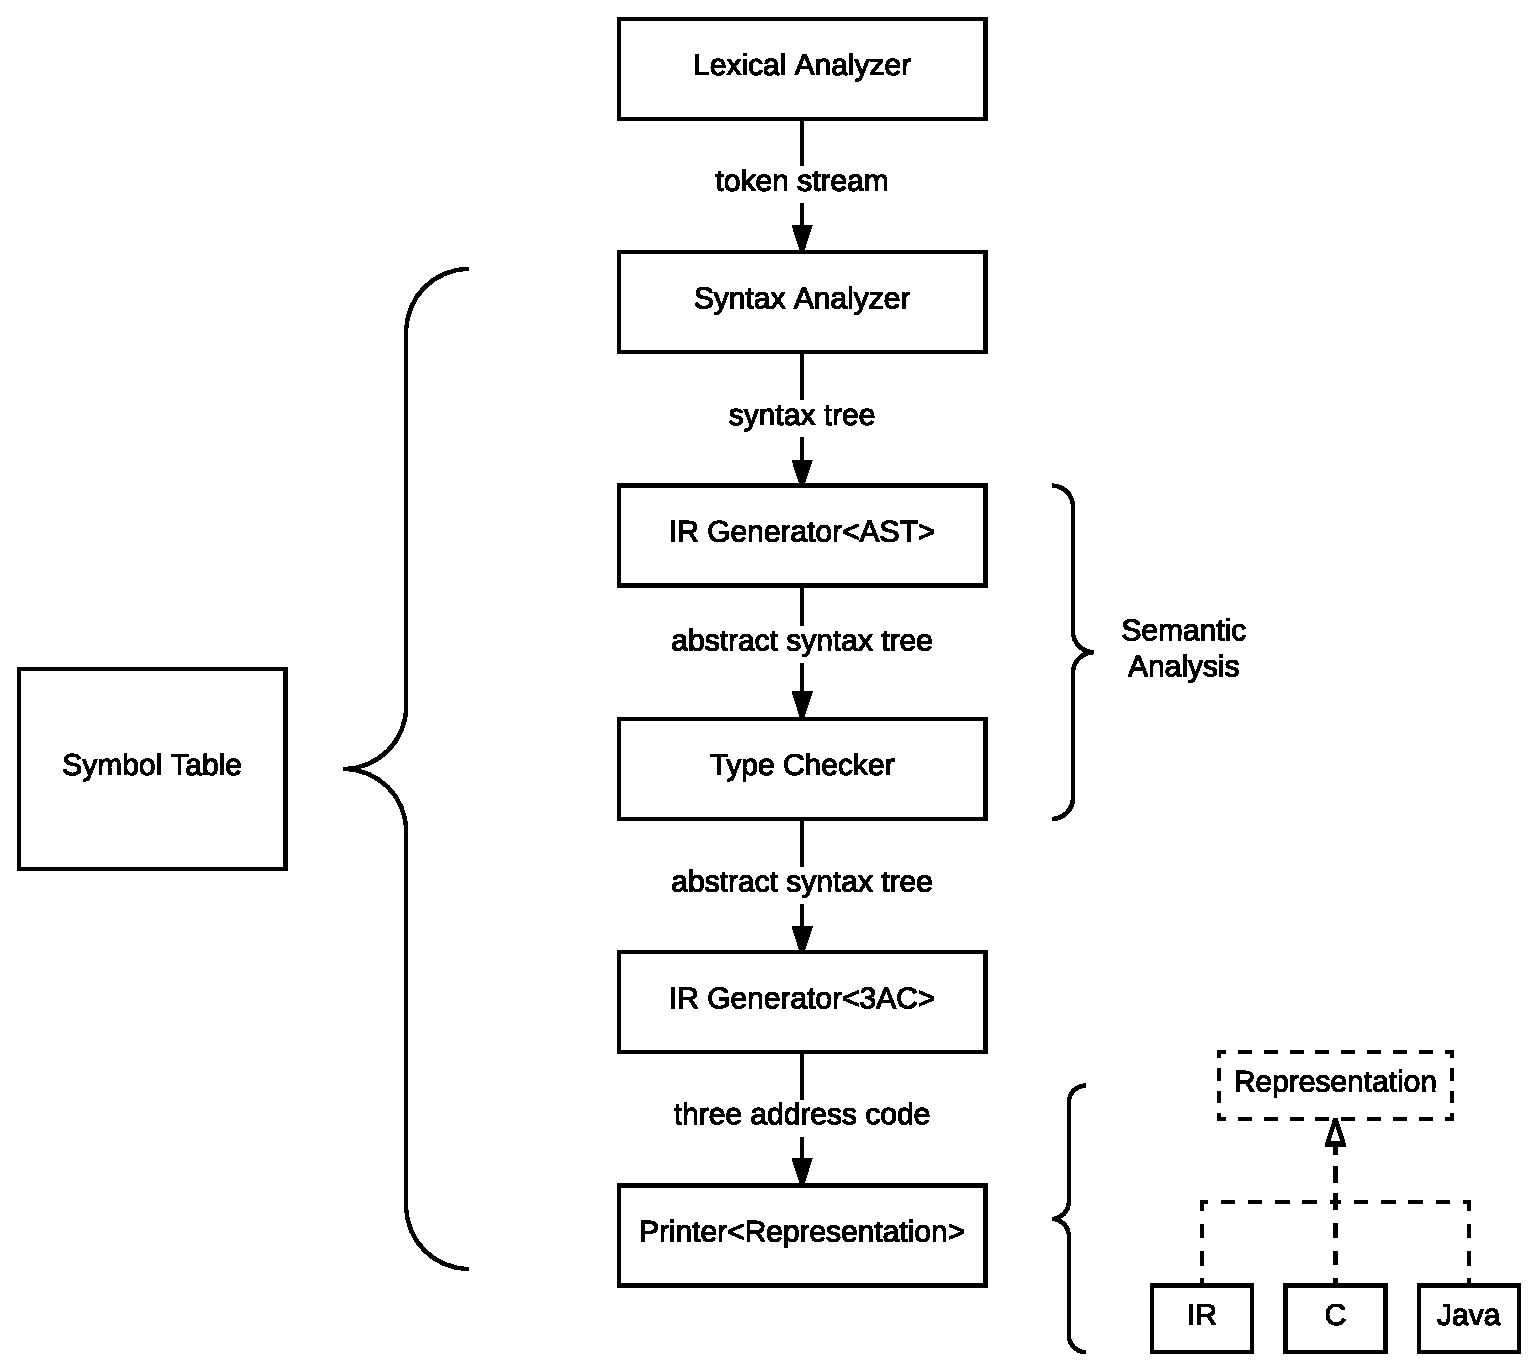
\includegraphics[width=.9\columnwidth]{img/eps/architecture.eps}
  \caption{Architectural Overview of the FAC compiler.}
  \label{fig:arch-ovw}
\end{figure}

\section{Lexer}
The lexical analyzer has been written using flex.
It has the following responsabilities:
\begin{itemize}
\item Verify that the input stream is lexically correct;
\item Produce the token stream for the parser;
\item Set the \verb|bison/flex| variable \verb|yylloc| -- this
variable contains the information about the first column, last column,
first row and last row of the token read. More details on its usage in
bison can be read in the bison section \ref{sec:parser}.
\item Raise an error in case of a fract constant with denominator equal
to $0$ -- it is simply not considered as a valid lexeme.
\end{itemize}


\subsection{Lexemes}
We chose to define an identifier for each lexem, this enable us to change the
syntax of the F language without affecting its semantics and the other
components. Basically, the goal of this choice is to have something similar to
a C macro or a placeholder for the syntax symbols of the F language.
For example we have defined \verb|SUM| which is a placeholder for \verb|+|, so
if tomorrow we decide to use \verb|plus| to perform the arithmetic sum we can do
it transparently to the rest of the FAC code. This provides a great flexibility
for lexer symbols.

\subsection{Comments}
We have also implemented the regex which checks the comments. So it is possible
write comments in the source code of F programs. They will be simply discarded
during the phase of lexical analysis.

\section{Parser}
\label{sec:parser}
The main goal of the parser written in bison is to check the
syntax correctness and to produce the Abstract Syntax Tree (AST).

\subsection{F -- Syntax choices}
We think that a language for students of the middle-school should be
statically typed and type safe; at the same time it should be easy to use.
Indeed, these requirements can help the student to learn how a simple
high-level language works by discriminating between the different types.
In particular, our minimal type system provides two completely unrelated types.


Thus, we discriminated between them by introducing specific type-related
operators. In particular we have defined some boolean operators
(in addition to the ones usually provided\footnote{e.g. in C++, Java}):
\begin{itemize}
	\item \verb|XOR| - exclusive or (syntactic sugar for the boolean disequality);
	\item \verb|<->| - logical biimplication (syntactic sugar for the boolean 
	equality);
	\item \verb|->| - logical implication (syntactic sugar);
\end{itemize}

The remaining operators are pretty similar to the ones provided by C.
There is only a slight difference: for the arithmetic disequality we have opted
for the Pascal \verb|<>| over the C \verb|!=|.

The syntactic symbols exist \emph{only} in the lexer. In the
rest of the program, i.e. in the parser and in the semantic analyser, we used
only internal representation of the operators. Therefore, each grammar
symbol can be safely replaced without affecting the correctness of FAC.

\subsection{Grammar}
We will not report the whole grammar but \emph{only} its peculiarities.
You can find the complete grammar at \path{FAC/src/parser/parser.y}.

\paragraph{Expressions}
In F you have two types of variables: fract and boolean.
Originally we distinguished two grammar rules, one for booleans and
one for the arithmetic expressions. Unfortunately, this distinction
lead to \verb|reduce/reduce| conflicts in bison.
Indeed one valid expression built by only one identifier could not be
classified by bison as a boolean or as an arithmetic expression.


So, we decided to simplify the grammar to allow also malformed expressions that
are correctly resolved during the type checking phase.

%\begin{verbatim}
%expr,e1, e2 ::= f | b | id | e1 AOP2 e2 | AOP1 expr | !expr | e1 BOP2 e2 | e1 RELOP e2
%\end{verbatim}

\paragraph{Declarations}

In order to avoid possible unitialized variables in the code, the grammar
forces the user to assign a value to a variable when declaring it.
Thus, the user proactively avoids possible C undefined behaviours.
This is a typical situation which can arise
when branching are involved, as depicted in the following example:
\begin{verbatim}
fract f;
while( BEXPR ) {
    // Do some stuff
    f = [1 | 3];
}
//is f initialized or not?
\end{verbatim}

\subsection{Error Handling}
We have redefined the standard \verb|yyerror| function provided by bison.
Our \verb|yyerror| implementation is variadic in order to accept any numbers of
arguments. Also, it frees the resources used during parsing before exiting with
failure code.

\section{Symbol Table}

\section{Type-Checking}
\label{sec:type-checking}

The type-checker receives as input the AST created by the 
parser. This data structure is convenient to perform
type checking because it gets rid of the syntactic symbols and also because it 
is easy traversable.
In our implementation each operator is wrapped into a category.
For instance the operators LT, LE, EQ, NEQ, GT, GE belongs to the category 
RELOP. So, we need only a type system rule for each operation of the category.
This makes the implementation of the type checker more readable.


As already mentioned, in our implementation we distinguish between two types:
boolean and fract. Each time a variable is declared its type is saved into the 
corresponding symbol table entry, thus facilitating the type checking.

So, we implemented a simple type system which exploits the symbol
table as the context. Each time a new variable is declared 
the context is updated with the new variable. This allows us to find whenever
a variable is used before its declaration.

\section{Three Address Code}
We chose to implement the indirect triples approach to represent internally
the three address code. As reported by the Dragon Book this representation 
can help in optimizing the resulting code, because the instructions can be 
easily swapped to improve the performances.

We generate the three address code starting from the AST, which does not contain
type errors.

\section{Conclusion}
\subsection{Difficulties encountered}
The implementation of the 3AC generator along with the C printer implementation 
(these components are related) have been the hardest part of the project. The 
difficulty was mostly due the lackness of a clear track to proceed. Indeed, we
had to choose how to build the 3AC specific implementation. Initially we tried
to implement a recursive version of the generator by passing the partial 3AC 
list to the successors and delegating the completion of a subtree 
(concatenating one or more lists) to the leaves. However, this approach was soon 
discarded because too complicated to implement. So, we decide to implement a 
recursive 3AC generator a bit more inefficient but a lot more clear and simple. 
Basically, the lists of the 3AC are constructed when returning from the 
recursive invocations and each composite case (e.g. if-then-else, assignment, 
etc.) handle its subtree (lists) connections.
\subsection{Future works}
\paragraph{Design}
To improve the current FAC front end design we think that a stronger decoupling 
of the components is necessary. The interfaces and their relationships are of 
fundamental importance for the development of the system. Currently, the code 
suffers from the god class anti pattern \cite{Martin:2008:CCH:1388398}. 
The parser concentrates too much dependencies and responsibilities inside 
itself. All the invocations to the AST generator, the type checker, the 3AC 
generator and the printer are performed by the parser! This problem was due to a
short-sighted design decision taken when we started building the parser. 
Unfortunately, proceeding with the project, we didn't find the time to refactor 
this component (the parser). Indeed, other components needed to be implemented 
in time to complete the project and to do not miss the deadline.

\paragraph{Features}
Other interesting features that could be implemented are:
\begin{itemize}
	\item scoped variables - automatically deallocated by the stack when they 
	go out of scope;
	\item first-class functions - a primitive type for function so they 
	can be used and also passed as parameters;
	\item pattern matching - provide a pattern matching feature to avoid using
	nested if-then-else and make code more clear;
	\item composite types - we found pretty interesting the lazy evaluated lists
	provided by Haskell;
	\item range types - this idea comes from R which lets you define a
	range of elements with 1 statement.
\end{itemize}
\bibliography{bib/bibliography}
\bibliographystyle{ieeetr}


\end{document}
